% !TEX root = ../thesis.tex

% Tässä osassa esitetään tulokset ja vastataan tutkielman alussa
% esitettyihin tutkimuskysymyksiin. Tieteellisen kirjoitelman
% arvo mitataan tässä osassa esitettyjen tulosten perusteella.

% You have done your work, but that’s1 not enough.
% You also need to evaluate how well your implementation works. The
% nature of the evaluation depends on your problem, your method, and your
% implementation that are all described in the thesis before this chapter. If
% you have created a program for exact-text matching, then you measure how
% long it takes for your implementation to search for different patterns, and
% compare it against the implementation that was used before. If you have
% designed a process for managing software projects, you perhaps interview
% people working with a waterfall-style management process, have them adapt
% your management process, and interview them again after they have worked
% with your process for some time. See what’s changed.
% The important thing is that you can evaluate your success somehow.
% Remember that you do not have to succeed in making something spectacular;
% a total implementation failure may still give grounds for a very good master’s
% thesis—if you can analyze what went wrong and what should have been done.

\documentclass[thesis.tex]{subfiles}

\begin{document}

\chapter{Experiment}
\label{chapter:experiment}

The purpose of the experiment was to investigate the feasibility and performance (precision) of photoluminescence-based product authentication using the fingerprint method described in the previous chapter. Additionally, another set of results was computed by replacing the fingerprint analysis and matching steps with a more computationally expensive histogram comparison approach (discussed briefly in more detail in Chapter \ref{chapter:results}). The following Chapter \ref{chapter:setup} introduces the luminophores, the hardware and the various capture, analysis and matching parameters used in the experiment. The results for both the fingerprint and the histogram method are summarized and compared in Chapter \ref{chapter:results}.

\section{Setup}
\label{chapter:setup}

The luminophores used in the experiment were LumiNova\textregistered\ red (O), green (G) and blue (DB) pigments. Each of the pigments was mixed with a transparent carrier to form a stock solution. The stock solutions were pipeted in increments of $50\mu l$ onto white blank cartons to form eight unique taggants. Two samples ($a$ and a replicate sample $b$) were taken from each solution, so a total of 16 different taggants were prepared for the experiment. The taggants and the amount of phosphor and transparent carrier used to create them are listed in Appendix \ref{appendix:taggants}. For information about the chemical properties of the LumiNova\textregistered\ pigments the reader is referred to \cite{luminova}.

The taggants were captured using Samsung S4 (version 4.4.2) and Lumia 1020 (version WP8.1) smartphones. The MFD of the S4 and the 1020 was determined empirically to be around 100mm and 150mm, respectively. The height of the camera module was adjusted accordingly to ensure that no image blur would be introduced. As depicted in Figure \ref{figure:camera_module} the light source was positioned perpendicular to the taggant as per the common conventions in fluorescense spectoscopy \cite{spectroscopy-principles}. Yongnuo YN565EX\footnote{Yongnuo YN565EX User Manual: \url{http://www.yongnuo.com.cn/usermanual/pdf/USER_MANUAL_YN565EX_EN.pdf}} external camera flash was used as the light source as it provided a convenient way to produce a high quality, full-spectrum white light for the photoexcitation. The power and zoom level of the flash were set to 1/32 and 24mm, respectively. The zoom level of the flash was set to the widest supported level assuming that the taggant would be more suspectible to uneven exposure on higher levels of zoom due to a more concentrated burst of light. The power level of 1/32 was selected by observing at which level the captured frames would no longer be overexposed.

The taggants were captured in a dimly lit room to minimize interference of ambient light. In total, nine different capture presets were defined: six presets ($an$) for the Samsung S4 and three presets ($wp$) for the Lumia 1020. The capture presets and the corresponding parameter values are listed in Appendix \ref{appendix:capture-presets}. The parameter values are discussed more thoroughly in Chapter \ref{chapter:discussion}. All of the 16 taggants were captured with each of the presets resulting in a corpus of 144 fingerprints (including $a$ and $b$ samples). After capture, each taggant was given 15 minutes to reset to ground state in order to minimize the effect of residual afterglow on subsequent captures. During the experiment the taggants were protected from any external sources of light to prevent exciting the luminophore prior to capture.

\section{Results}
\label{chapter:results}

Various possible configurations (permutations), vast amount of data. Thus, top down approach. Broad level results -> some peculiar cases


5 Analysis \& matching parameters

- binary thresholding: threshold value 40 => filter dark pixels (brightness less than 15\%)
- peak valley delta (PVD) 0.2
- similarity parameters (damping...)

Results storyline:

assumption is that the lowest score is the b sample

- comparison vs. histogram approach
- Clusters to indicate pipeline accuracy on a broad level (why AP clustering?)
  - Run similarity matrix through affinity propagation (R's aPCluster) / dimensionality reduction
  - Bhattacharyya distance (why?)
  - the more clusters the better
  - We want clusters that...
    - dont include too many/few taggants (preferably 3-6)
    - are equal in value (y-axis)
    - are of the same/similar color
- Margin 10, 15 and 25\% to indicate histogram > fingerprint method (=> focus on histogram method)
- Evaluate the effect of capture (/analysis) params
  - ignore resolution, look at interval?
  - find anomalies
  - visualize which taggants perform the best, and why? (good match: an\_600/24SPa, an\_600\_r/24VPb)
- present artefacts
- boundary conditions: max margin and max count

\begin{figure}[h]
\centering 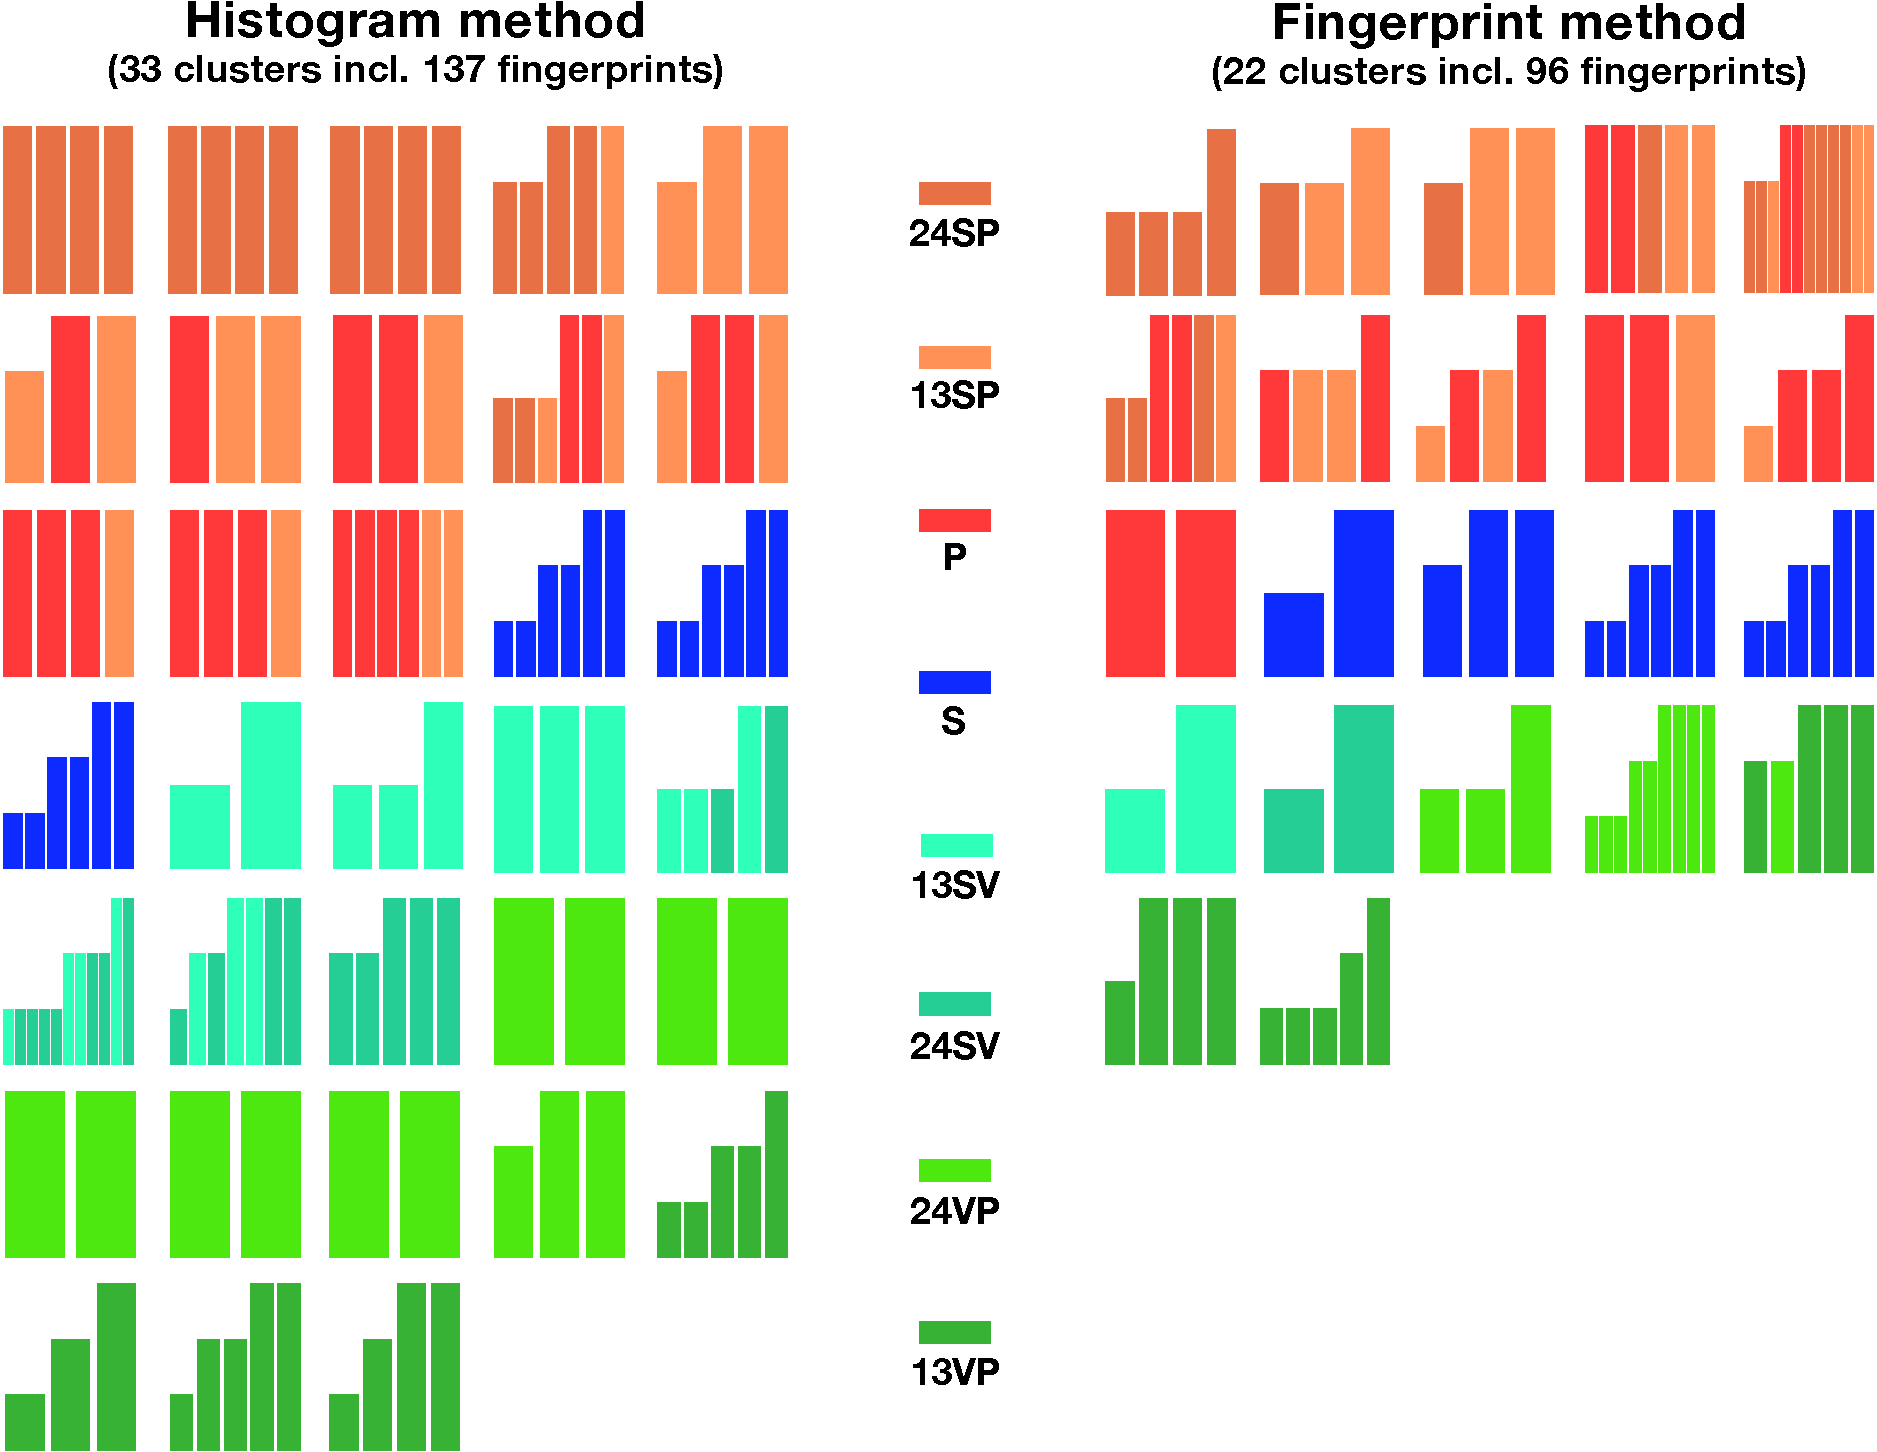
\includegraphics[page=1,width=\textwidth,height=\textheight,keepaspectratio=true]{images/experiment/clusters}
\end{figure}
\begin{figure}[h]
\centering 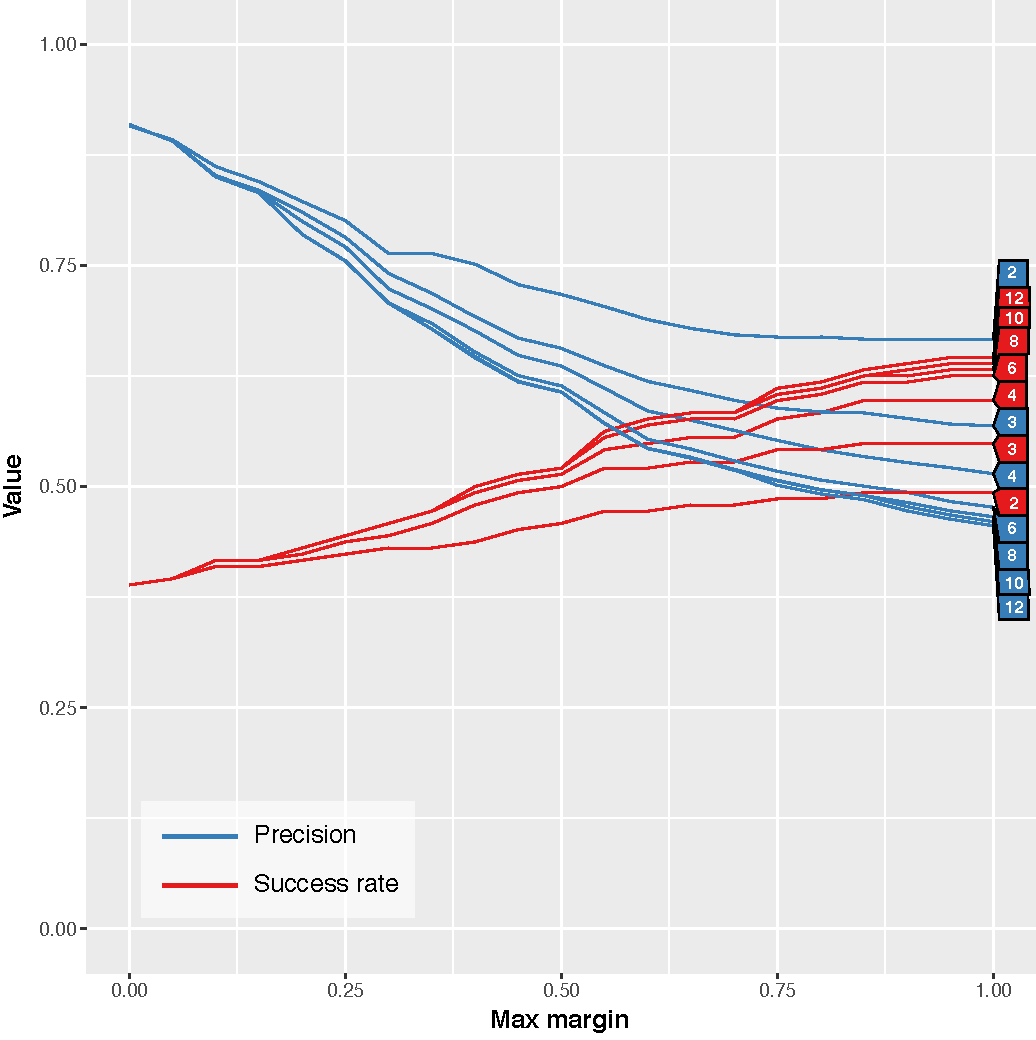
\includegraphics[page=1,width=\textwidth,height=\textheight,keepaspectratio=true]{images/experiment/match_precision}
\end{figure}
\begin{figure}[h]
\centering \includegraphics[page=2,width=\textwidth,height=\textheight,keepaspectratio=true]{images/experiment/match_precision}
\end{figure}
\begin{figure}[h]
\centering \includegraphics[page=3,width=\textwidth,height=\textheight,keepaspectratio=true]{images/experiment/match_precision}
\end{figure}
\begin{figure}[h]
\centering \includegraphics[page=7,width=\textwidth,height=\textheight,keepaspectratio=true]{images/experiment/tags_configs}
\end{figure}

\end{document}